\documentclass[12pt, twoside]{article}
\usepackage[letterpaper, margin=1in, headsep=0.5in]{geometry}
\usepackage[english]{babel}
\usepackage[utf8]{inputenc}
\usepackage{amsmath}
\usepackage{amsfonts}
\usepackage{amssymb}
\usepackage{tikz}
%\usetikzlibrary{quotes, angles}

\usepackage{graphicx}
\usepackage{enumitem}
\usepackage{multicol}

\usepackage{fancyhdr}
\pagestyle{fancy}
\fancyhf{}
\renewcommand{\headrulewidth}{0pt} % disable the underline of the header

\fancyhead[R]{\thepage}
\fancyhead[L]{BECA / Dr. Huson / 10th Grade Geometry\\* Learning trajectory: Trigonometry}

\begin{document}
\subsubsection*{Trig}
  \begin{enumerate}
    \item Slope as $\tan \theta$
    \item calculate sine, cosine, tangent from diagram
    \item Calculator use, finding missing sides
    \item Find angle value using inverse function
    \item Angle of elevation, depression, declination, incline (in Regents scope?)
    \item Word problem interpretation
    \item Sine and cosine are cofunctions, explain and apply
  \end{enumerate}

  \begin{enumerate}
    \subsubsection*{Diagrams}
    \item Sine and cosine

  \item Sine and cosine are cofunctions, explain and apply\\
  Given the right triangle $ABC$ with $m\angle C=90^\circ$. If $\sin A$ increases, will $\cos B$ increase, decrease, or stay the same? Explain why.\\
  Draw a right triangle, labeling vertices with capital letters and opposite sides with small letters. Write down the trig functions as ratios, explaining that they are equal.
  \end{enumerate}

\newpage

\subsubsection*{Regents trigonometry problems}
  \begin{enumerate}
  \item Round to \emph{the nearest tenth} of a meter.\\
  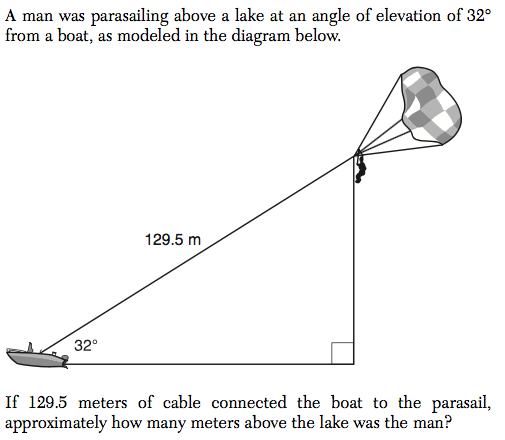
\includegraphics[width=0.7\textwidth]{trig-boat.png} \vspace{3cm}
  \item Solve for $x$.\\
  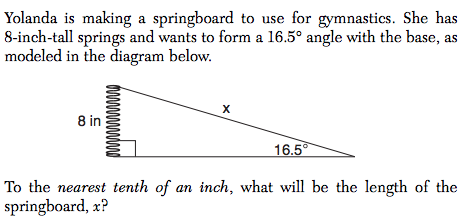
\includegraphics[width=0.7\textwidth]{trig-spring.png}
  \end{enumerate}


\end{document}
